\chapter{Pojazdy UAV i systemy AVS}
\label{cha:Pojazdy_UAV_i_systemy_AVS}
%---------------------------------------------------------------------------
\section{Pojęcia}
\label{sec:Pojecia}
Systemy AVS (\textit{Aerial Video Surveillance}, z ang. systemy powietrznej obserwacji), czyli systemy umożliwiające obserwację obiektu zainteresowania z pokładu pojazdu latającego z wykorzystaniem urządzenia rejestrującego obraz, od dawna znajdują zastosowanie w technice militarnej i cywilnej. Wachlarz ich zastosowań jest szeroki - jako przykłady można podać śledzenie aktywności wrogich jednostek wojskowych, obserwację przeciwpożarową, nadzorowanie ruchu drogowego czy przeprowadzanie działań bojowych. Obecnie rozwój rynku i technologii pojazdów UAV (\textit{Unmanned Aerial Vehicle}, z ang. bezzałogowe pojazdy latające), w których montowane są systemy AVS jest najbardziej dynamiczny w jego dotychczasowej historii. Według prognozy wykonanej przez \textit{Market Research Media Ltd.} \cite{MarResMedUAVMarket} wartość tylko amerykańskiego rynku pojazdów UAV w 2018r. wyniesie 18,7 bilionów dolarów.

\begin{figure}[!htb]
	\centering
	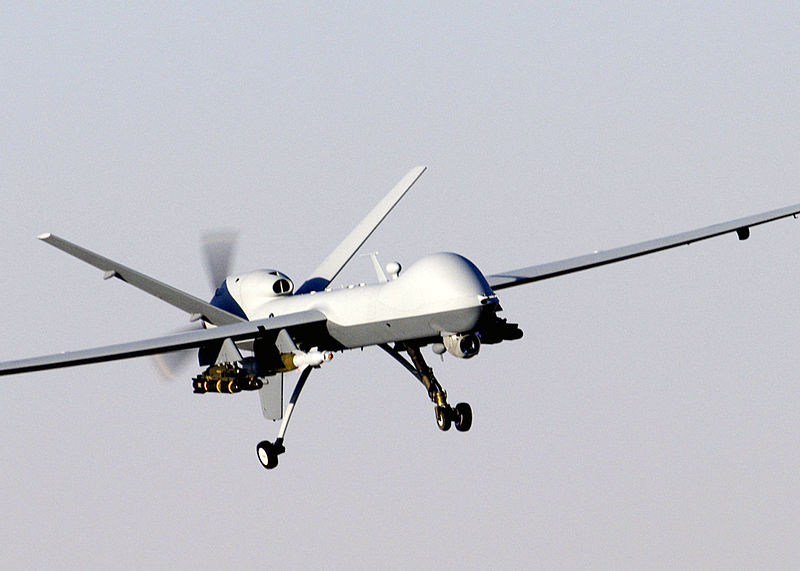
\includegraphics[width=8cm]{Images/MQ9_reaper_enwikipediaorg.jpg}
	\captionsource{Pojazd UAV MQ-9 Reaper}{\url{http://en.wikipedia.org/wiki/File:MQ-9_Reaper_in_flight_\%282007\%29.jpg}}
	\label{img:MQ9_Reaper}
\end{figure}

Historia systemów AVS jest długa (jej początki sięgają XIX wieku) jednak ich zastosowanie w pojazdach UAV przyczyniło się do rozwoju i zmiany ich formuły. Współczesne systemy AVS stanowią element składy układu sterowania pojazdów UAV, umożliwiając ich coraz dalej postępującą automatyzację.
Jako typowe funkcje systemów AVS można wymienić:
\begin{enumerate}
\item Wykrywanie i śledzenie poruszającego się obiektu naziemnego
\item Geo-lokalizacja wykrytych obiektów
\item Tworzenie map terenu
\item ...
\end{enumerate}